\documentclass[a4paper,10pt]{ltjsarticle}

% プリアンブル
%\usepackage[dvipdfmx]{graphicx}
%\usepackage[dvipdfmx]{color}
\usepackage{graphicx}
\usepackage{color}
\usepackage{amsthm}
\usepackage{amsmath}
\usepackage{amsfonts}
\usepackage{mathtools}
\usepackage{listings}
\usepackage[dvipdfmx]{hyperref}
\usepackage{here}
\usepackage{amssymb}
\usepackage{algorithmic}
\usepackage{algorithm}
\usepackage{bbm}
\usepackage{caption}
\usepackage{fancyhdr}
\pagestyle{fancy}
\lhead{Survey by D. Nishiyama on \today}    % ヘッダの右側
%\cfoot{\thepage}                % フッター中央
\renewcommand{\headrulewidth}{0pt}        % ヘッダの線の太さ:0ptで消える

\newcommand{\bi}[1]{\ensuremath{\boldsymbol{#1}}}
\newcommand{\multicell}[2]{\begin{tabular}{c}
                               #1\\#2
\end{tabular}}


% 転置記号
\newcommand{\T}{\ensuremath{^{\text{T}}}}

% 図の参照
\newcommand{\Zu}[1]{図\ref{fig:#1}}

% 表の参照
\newcommand{\Hyou}[1]{表\ref{tab:#1}}
\newcommand{\II}{I\hspace{-.1em}I}
% 式の参照
\newcommand{\Shiki}[1]{式\eqref{eq:#1}}
\newcommand{\1}{\mbox{1}\hspace{-0.25em}\mbox{l}}
\lstset{
    basicstyle={\ttfamily\small}, %書体の指定
    frame=tRBl, %フレームの指定
    framesep=10pt, %フレームと中身(コード)の間隔
    breaklines=true, %行が長くなった場合の改行
    linewidth=15cm, %フレームの横幅
    lineskip=-0.5ex, %行間の調整
    tabsize=2 %Tabを何文字幅にするかの指定
}
\usepackage{multirow}
\usepackage{stmaryrd}
\usepackage{subfiles}
\theoremstyle{definition}
\newtheorem{theorem}{定理}
\newtheorem*{theorem*}{定理}
\newtheorem{prop}{命題}
\newtheorem*{prop*}{命題}
\newtheorem{definition}[theorem]{定義}
\newtheorem*{definition*}{定義}

\def\hlineb{%
    \noalign{\ifnum0=`}\fi\hrule \@height \arrayrulewidthb \futurelet
    \reserved@a\@xhlineb}
\def\@xhlineb{\ifx\reserved@a\hlineb
\vskip\doublerulesep
\vskip-\arrayrulewidthb
\fi
\ifnum0=`{\fi}}

\newcommand{\argmax}{\mathop{\rm arg~max}\limits}
\newcommand{\argmin}{\mathop{\rm arg~min}\limits}
\title{Notes on the Overview}
\author{D. NSYM}
\date{\today}

%!  心構え
%!  ・時間を決めて読む
%!  ・まとめる癖をつける


%! 読む順番 パターンA(じっくり)
%!  1.アブストラクト(何をしたか)、イントロダクション(何をしたいか)
%!  2.結論(何をしたか・詳細)
%!  3.実験結果(主張の証明)・議論(良し悪し)
%!  4.関連研究(他との違い)、メソッド(実験方法)

%! 読む順番 パターンB(ざっくり)
%!  1.アブストラクト(何をしたか)
%!  2.イントロダクション(何をしたいか)
%!  3.結果(主として図)
% Document
\begin{document}
    \maketitle

    説明法とは、ユ一ザが欲しい追加情報を機械学習モデルから抽出する技術。
    『どんな追加情報が欲しいか』はデータ/応用によって異なる。
    仮説に基づいて鮵明法の研究開発を進めていることが多い。


    \section{CNN向けの説明手法・フレームワーク}

    \subsection{Grad-CAM\cite{selvaraju2017grad}}

    最後のconvolutional layerからの勾配のヒートマップを生成することによって視覚的な説明を提供。

    Grad-CAMでは、最終的な畳み込み特徴マップに対する分類スコアの勾配を利用して、分類スコアに最も影響を与える入力イメージの部分を識別する。
    この勾配が大きくなる場所は、最終的なスコアがデータに最も依存する場所を示す。

    \subsection{LIME\cite{ribeiro2016should}}

    解釈可能なモデルを局所的に学習することで、任意の分類器や回帰の局所的に忠実な説明を生成する
    \begin{itemize}
        \item どの特徴が予測に重要だったかを提示する。
        \item モデルを説明対象データの周辺で線形モデルで近似する。
        \item 線形モデルの係数の大小で, 各特徵の重要度合いを測る。
    \end{itemize}
    \begin{figure}[H]
        \centering
        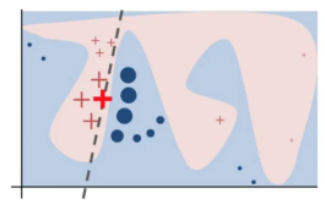
\includegraphics[width=80mm]{fig/lime}
        \caption{LIMEの概要}
    \end{figure}

    \subsection{ProtoPNet\cite{chen2019looks}}
    モデルの性能を犠牲にすることなく、
    画像中のプロトタイプの部品を識別できるprototypical part network(ProtoPNet)を提案
    \begin{enumerate}
        \item 深層特徴抽出モジュール$f$で、入力画像の一部の領域を表現する特徴ベクトル$x$を得る
        \item $f$で訓練画像の一部の領域を表現する特徴ベクトル$x^\prime$を得て、プロトタイプ:訓練データの代表点とする
        \item 入力画像の各領域$x$と訓練画像の代表領域$x^\prime$との類似度を評価し、各領域間の類似度\bi{S}を得る
        \item \bi{S}を入力に取る線形予測モジュール$L$で識別。$L$の重み$w_{mk}$の大きさは、入力画像の$m$番目の領域と訓練画像の$k$番目の領域が似ていることが予測に影響していることを意味する。
    \end{enumerate}
    \begin{figure}[H]
        \centering
        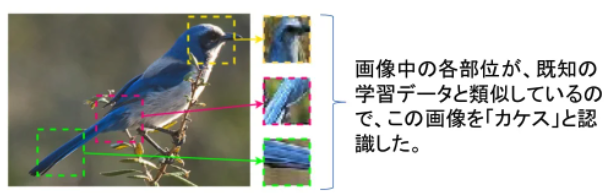
\includegraphics[width=120mm]{fig/protopnet}
        \caption{ProtPNetの概要}
    \end{figure}
    \begin{figure}[H]
        \centering
        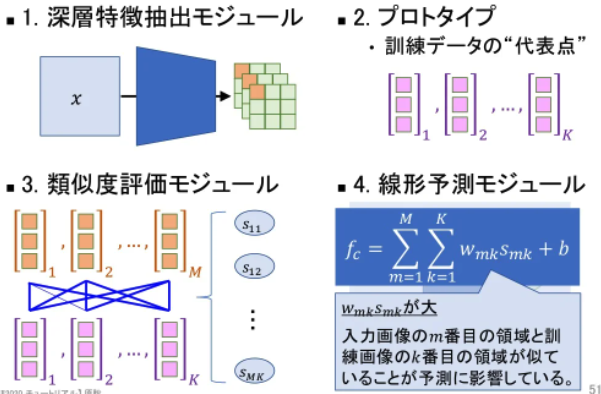
\includegraphics[width=80mm]{fig/protop_2}
        \caption{ProtPNetの仕組み}
    \end{figure}



    \bibliographystyle{apalike}
    \bibliography{/Users/funami/Documents/Survey/ref}
\end{document}

